%%TITRE
\begin{center}
    \textbf{\Large OPTIMIZATION IN INDUSTRY - J. DARLAY} \\
    \vspace{0.5cm}

    Miniconference Report \\
    CHAU Dang Minh
\end{center}

\begin{center}
    \begin{minipage}{0.85\textwidth}
        \textbf{Summary.} Dr. J. Darly, the Head of Science at Hexaly Company, gave an introduction to optimization in industry, including how such kind of optimization differs from academic one, and introduced Hexaly's optimization language for a particular problem.
    \end{minipage}
\end{center}

\vspace{1cm}


In the heart of academic optimization theory lies popular problems, such as linear regression, support vector machine and decision tree. When applying these problems into industrial problems, a scientist or engineer has to choose and combine based on a large amount of mathematical properties in order to ensure tractability, runtime constraints, business constraints, scalability and maintainability. Moreover, the problem definition can also change. Examples of such problems include Audience forecast (TF1), Telecom user behavior, and Failure prediction.

In the algorithmic approach, the first step is modelling, with an aim to understand the problem, find the objectives, variables and constraints, as well as define an appropriate mathematical model for the problem. The second step is solving. Usually, the priority is not an optimal solution, but to define what a good bound and a good solution are, then attempt to find a satisfying solution. Due to the nature of an industrial optimization problem, such approach is not suitable, since these time-consuming steps have to be completely run for every new problem, despite the fact that some problems may have some similar patterns. Therefore, the business approach is to create an optimization language and solvers.

An optimization language, AMPL, has been studied in the course of Practical Optimization, consisting of data, a model and a solver script. Hexaly's language also serves the same concepts but more user friendly. The syntax is similar to that of Python. A program contains the following main functions. The \textit{input} function is used to transform the data into a desired format. The \textit{model} function is used to define the objective and constraints. Finally, the \textit{output} function is used to transform the solution to a desired format. However, as in the introduction, the solver is built-in and cannot be defined precisely, which may be to preserve authenticity. A simple program has been written in this language in order to solve the \href{https://www.kaggle.com/c/santa-workshop-tour-2019}{Santa's Workshop Tour Problem}. After solving the problem, it can be discovered that Hexaly provides good infrastructure, since 14 million iterations were completed in just 35 seconds. A sample of the program is provided in Figure \ref{fig:sample}. The development of the interactive environment is also worth appreciating, since it lets programmers focus on the optimization deed and gives good feedback in the progress.

\begin{figure}[ht]
    \centering
    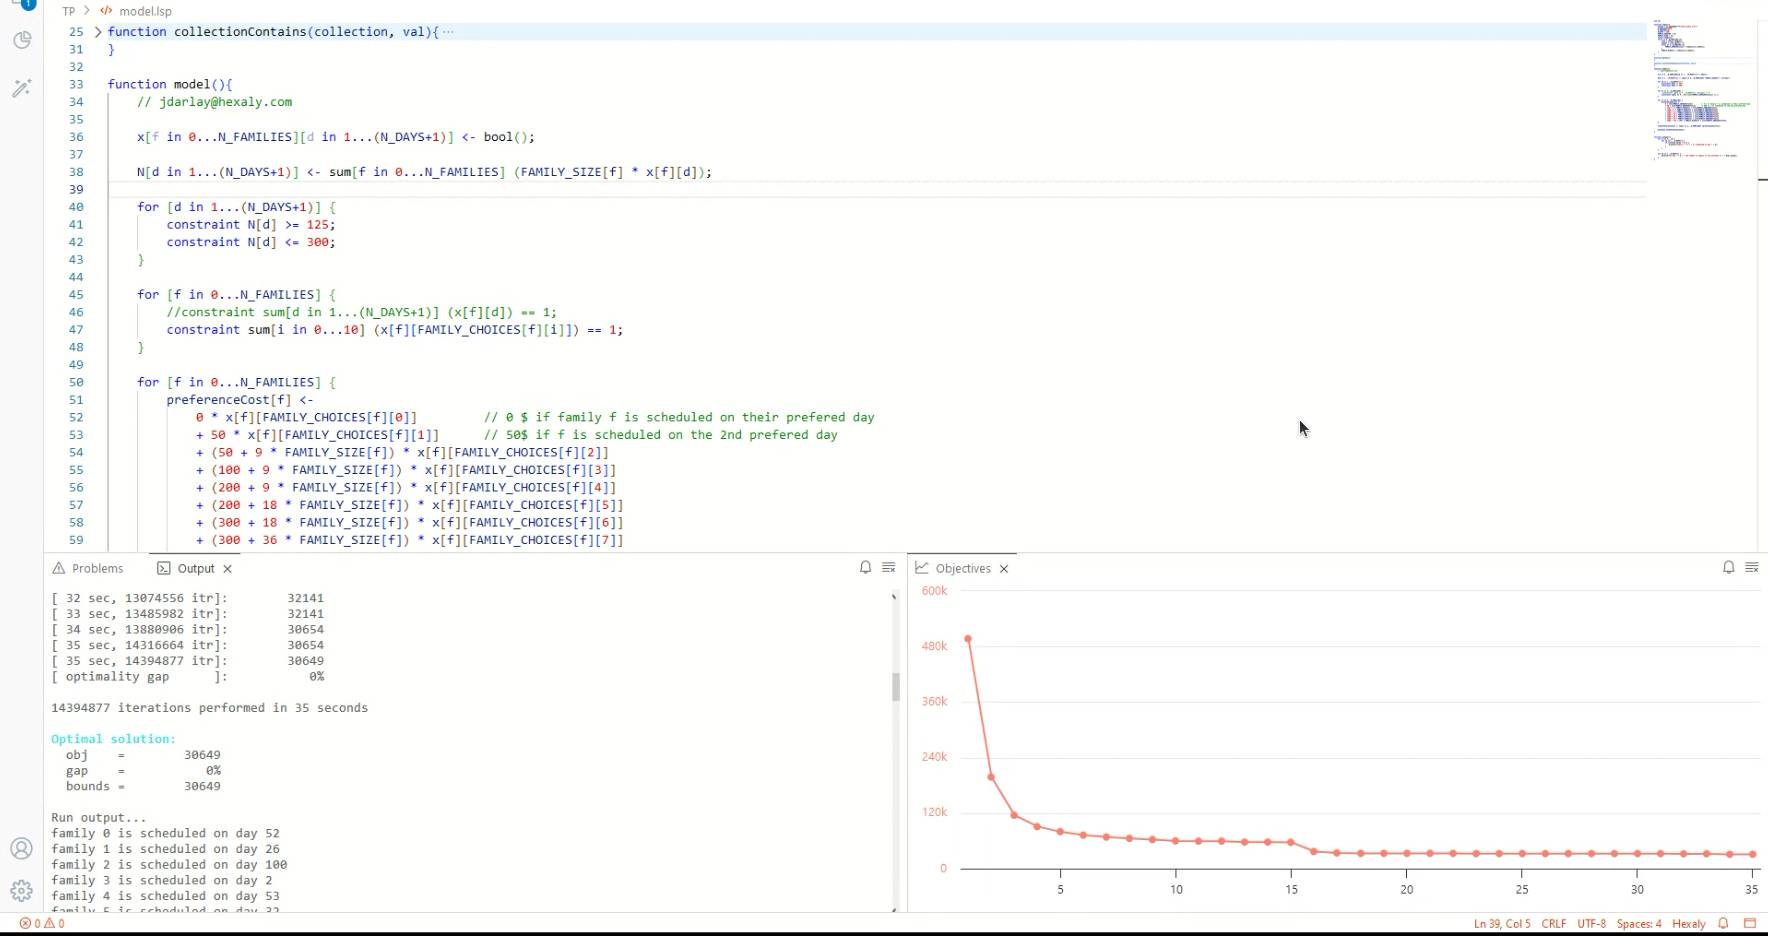
\includegraphics[width=\textwidth]{img/code.png}
    \caption{Sample code}
    \label{fig:sample}
\end{figure}

No matter if a master student pursues a career in academic or industry, and if they want to be specialized in the field of optimization, optimization problems are always a part of their work. Except for few number of publications on theoretical foundations, comparing to the number of publications on the improvement of approaches for new real-life problems, every publication on such improvements can be considered as a solution to an optimization problem. Even in a foundational field such as logic, since undecidability has been discovered, researchers have been aiming to provide tractable partial solution. Therefore, Dr. J. Darly's lecture on industrial optimization is valuable for us master students. It reminds us the role of a general progress, rather than solving each problem individually as well as arising problems in real business. Then come optimization languages as an effort to implement them.
